\documentclass{article}

\usepackage[a4paper]{geometry}
\usepackage{graphicx}
\usepackage{multicol}
\usepackage{amssymb}

\usepackage{xspace}
\usepackage[pdftex]{hyperref}
\usepackage[usenames,dvipsnames]{color}
\usepackage{verbatim}

%macros
\newcommand{\SSm}[2]{SuffSmall(#1,#2)}
\newcommand{\p}[2]{pair(#1,#2)}

%definitions
\def \DH{David Hirsch\xspace}
\def \A{Attribute\xspace}

% Attribute Sections
\def \AS{\A Catagories\xspace}

\def \OC{Optical Character\xspace}
\def \GS{Grain Shape\xspace}
\def \IRF{Index of Refraction\xspace}
\def \Col{Pleochroism\xspace}
\def \C{Cleavage\xspace}
\def \T{Twinning\xspace}
\def \B{Birefringence\xspace}
\def \Ab{Abbundance\xspace}

\def \OCc{SpringGreen}
\def \GSc{OliveGreen}
\def \IRFc{SkyBlue}
\def \Colc{Tan}
\def \Cc{Thistle}
\def \Tc{Melon}
\def \Bc{Yellow}
\def \Abc{RedViolet}

%Attribure Types
\def \AT{\A Types\xspace}
\def \ColA{Color Attribute\xspace}
\def \EnumA{Enumerated Attribute\xspace}
\def \RangeA{Range Attribute\xspace}
\def \PruneA{Prune Attribute\xspace}
%
\def \cv{CV}

%enumerated
\def \cs{cleavage\_shape\xspace}
\def \twt{twin$_i$\_type\xspace}
\def \to{true\_optics\xspace}
\def \op{opaque\xspace}

%prune
\def \rt{rock\_type\xspace}

%integer range
\def \tvx{twovx\xspace}
\def \cn{cleavage\_num\xspace}
\def \bl{blasticity\xspace}
\def \ca{cleavage\_angle\xspace}
\def \ds{dispersion\_strength\xspace}

%floating range
\def \arzy{aspect\_ratio\_zy\xspace}
\def \arxy{aspect\_ratio\_xy\xspace}
\def \ira{index\_of\_refraction$_\alpha$\xspace}
\def \irb{index\_of\_refraction$_\beta$\xspace}
\def \irc{index\_of\_refraction$_\gamma$\xspace}
\def \b{birefringence\_num\xspace}

%color searches
\def \plcola{pleochroism\_col$_1$\xspace}
\def \plcolb{pleochroism\_col$_2$\xspace}
\def \plcolc{pleochroism\_col$_3$\xspace}

\def \aic{anomalous\_interference\_col\xspace}

\def \FP{{\bf False Negative}\xspace}

\title{Scoring Document}
\date{Last Edited - \today}
\begin{document}
\maketitle
For this review, we will be using 
\begin{itemize}
\item \SSm{A}{x} to denote the conditional that for attribute A and numerical x, $(A\leq x)$.
\item \p{R}{S} to denote a paired information relationship
\end{itemize}


\section*{Domain and Range}
We have a growing number of Minerals with a finite number of attributes that are tied to these minerals. It is our concern to design a (search/scoring algorithm) and (database) which with as little deviance as possible addresses the Attributes as our domain for retrieving minerals. 


\begin{tabular}{|l|l|l|l|}
  
  {\bf\em Floating Point}&{\bf\em Integer}&{\bf\em Enumerated}&{\bf\em Color}\\
   \hline
   { \colorbox{\GSc} \arzy }&{ \colorbox{\OCc} \tvx }&{ \colorbox{\Cc} \cs }&{ \colorbox{\Colc} \plcola }\\
   { \colorbox{\GSc} \arxy }&{ \colorbox{\Cc} \cn  }&{ \colorbox{\Tc} \twt }&{ \colorbox{\Colc} \plcolb }\\
   { \colorbox{\IRFc} \ira }&{ \colorbox{\Cc} \ca  }&{ \colorbox{\OCc} \to  }&{ \colorbox{\Colc} \plcolc }\\
   { \colorbox{\IRFc} \irb }&{ \colorbox{\GSc} \bl  }&{ \colorbox{\OCc} \op  }&{ \colorbox{\Bc} \aic    }\\
   { \colorbox{\IRFc} \irc }&{ \colorbox{\Bc} \ds  }&{ \colorbox{\Abc} \rt  }&         \\
   { \colorbox{\Bc} \b     }& &  & \\
\end{tabular}
   
\section*{\AS}
There are several different \AS. The \AS are divided by overall topic and are made openly apparent in the UI. 

\begin{multicols}{2}
\begin{enumerate}
\item {\colorbox{\OCc} \OC}
\item {\colorbox{\GSc} \GS}
\item {\colorbox{\IRFc} \IRF}
\item {\colorbox{\Colc} \Col}
\item {\colorbox{\Cc} \C}
\item {\colorbox{\Tc} \T}
\item {\colorbox{\Bc} \B}
\item {\colorbox{\Abc} \Ab}
\end{enumerate}
\end{multicols}

These are sectioned off in the UI by topic, this does not imply a lack of relation between data retrieved within differing \AS, It is only a model of organizing for user ease.

\section*{\AT}
The greater concern for our database operations is the \AT. Every unique type must have a slightly different search algorithm. Listed are the currently identified.

\begin{enumerate}
\item \ColA
\item \EnumA
\item \PruneA
\item \RangeA
\end{enumerate}

%\label{marker}\hyperref{ name \ref*{marker}}

\subsection*{\ColA}
We have two major themes for searching colors in the database. After bringing these two methods to \DH's attention, he asked us to focus on other \AT more so the documentation on this \AS will be brief. For this category we are currently assuming that the colors are stored and addressed as HTML Color codes. We also note for full disclosure that in the mineral structure for every color there exists a variability number that we will call the \cv stored in hexadecimal form.


\subsubsection*{Method 1}
The first option for color identification is to allow a user to select from a standard color picker like the one \url{"http://www.colorpicker.com/"}. The Color-Picker layout is not important as long as it is continuous gradient for this model.

\begin{center}
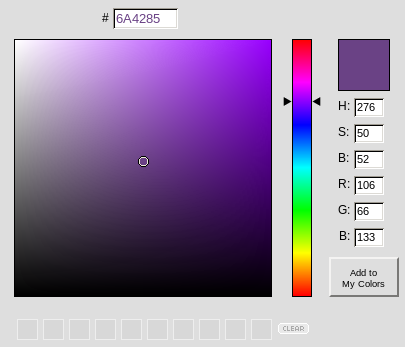
\includegraphics[width=60mm]{colorpicker.png}
\end{center}

It is the algorithm's job determine if the user's input \#XXYYZZ color code is in each minerals \#QQRRSS range as defined by the area in \#QQRRSS - \#\cv{}\cv{}\cv x \# QQRRSS+\#\cv{}\cv{}\cv. The computational cost of this operation is rather heavy, and the user could easily choose a color that is outside of all of these values because they are provided to him, however it is more likely that the user is happy with their choice.

\subsubsection*{Method 2}
The second proposed approach to this problem is to create images displaying the greatest of overlapping domains in color areas of the minerals. For this I will use an example:

\def \ma{Mineral$_1$\xspace}
\def \cva{\cv$_1$\xspace}
\def \mb{Mineral$_2$\xspace}
\def \cvb{\cv$_2$\xspace}

\begin{itemize}
\item[] given \ma with color code \#LLMMNN and \cva
\item[] given \mb with color code \#QQRRSS and \cvb
\end{itemize}

If the area of 
\begin{itemize}
\item[] \{\#LLMMNN $\pm$ \#\cva{}\cva{}\cva{}\} overlaps sufficiently with 
\item[] \{\#QQRRSS $\pm$ \#\cvb{}\cvb{}\cvb{}\} 
\end{itemize}
then they will be represented in the same color blot, and both minerals will be scored equally. This method forces the user to select an \emph{active} color region (if they are to choose a color) and allows categorical computations to happen prior to search cutting run time dramatically. 

\subsection*{\EnumA}
The enumerated types can easily be used for pruning in the general case, however there are certain combinations of attributes that will cause \FP in user categorization. The enumerated search variables are as listed:
\begin{enumerate}
\item \to
\item \cs
\item \twt
\end{enumerate}
These are relatively static, but contain several logical conditions in searching. 
\subsubsection*{\to}
Bellow is listed situations that result in incorrect guesses with respect to \to.
\scriptsize

\def \iso{isotropic\xspace}
\def \uni{uniaxial\xspace}
\def \bia{biaxial\xspace}
\begin{itemize}
\item The \to attribute has one of three options : \iso, \uni, \bia.
\item If \SSm{\b}{.005} and (\to == \iso) then (\to = \uni or \bia) are marked \FP
\item If \SSm{\b}{.005} and (\to == \uni) then (\to = \iso) is marked \FP
\item If \SSm{\tvx}{$10^\circ$} and (\to == \uni) then \to = \bia is marked \FP 
\item if \SSm{\tvx}{$10^\circ$} and (\to == \bia) then \to = \uni is marked \FP 
\end{itemize}


\normalsize
\subsubsection*{\cs}
\def \cub{cubic\xspace}
\def \oct{octahedral\xspace}
\def \rho{rhobohedral\xspace}
\cs is a parameter that is mutually search-able with \cn. Only one may be searched by a user. If they choose \cs it is assumed that they are more confident in their decision. 
\small
\begin{itemize}
\item \cub
\item \oct
\item \rho
\end{itemize}
\normalsize
\subsubsection*{\twt}
I have nothing to say here. I do not know if there are any unique issues with respect to assessing this enumerated type. \DH should be questioned on this.
 
\subsection*{\PruneA}
\def \occ{world\_occurrence\xspace}

The majority of the \PruneA{}s are found in \Ab. These types are the last evaluated, and are used to scale active scores before displaying to the user. Ideally this grants common minerals, greater scores and more rare minerals lesser relative scores. There are a few ways to handle this procedure, and each has its merits. 

%\subsubsection*{Simple - Default}
he simple approach, and default approach. The only Prune Attribute that is search-able is \rt. This is also the only search-able value in the \Ab Category. This allows users to put in the type of rock they are inspecting to more accurately weight their returned values. The algorithm is generalized so if users don't choose \rt the weights are drawn from (\occ $\in$ \Ab). [\occ is the \% of the earth that represents a given mineral ].

%\subsubsection*{Issue w/ Simple Default}
\def \fl{Fluorite\xspace}
\def \qu{Quartz\xspace}
A scenario that easily raises an issue: The user is identifying a rare mineral like \fl which has an \occ of 2\%, whose query also returns \qu at 75\%. If the scores provided for \fl and \occ were scaled linearly, as  percentages are expected to, it is likely that \qu would win out, even if \fl were a better match, unless \qu was a significantly lesser match. {\em Proposed solutions to this are :}
\def\scr{{\bf scatter plot representation}\xspace}
\begin{enumerate}
\item \scr
\item nonlinear scale - (perhaps logarithmic)
\item ability to disable score pruning
\item Secondary Sorting
\end{enumerate}

The \scr removes the responsibility of pruning from the programmer. It would display as an x-axis the \rt frequency ratings wrt returned minerals, and a y-axis of the scores they received. This allows the user to clearly identify where their mineral falls in it's worldly distribution. It's failing point would be when too many rare minerals are scored highly, the user would never receive high frequency minerals.

\subsubsection*{Alternatives for \PruneA}
We have not enough data to test this method out, however it is possible that using logarithmic scale to the mineral's \PruneA{}s would mellow out high scores enough to make the presented issue less relevant.

Disabling score pruning is by far the simplest means to implement, this lets the user decide what is more important. It also takes the responsibility out of the programmer for coming up with something clever. However, it is fair to argue that this should be a feature of the UI regardless.

The theme for secondary sorting is to identify highest scores first, separate sorted results into sections, then sort given sections using the \PruneA{}s.

\newpage
\subsection*{\RangeA}
The focus of our algorithm addresses \RangeA{}s. \RangeA{}s are individually searched with a 3:2 ratio. The user inputs their best guess, then provides a upper and lower bounds to their guess. This allows for much of the approximation to be the user's responsibility. 
\newline
\newline
\tiny

\begin{tabular}{l|l|l|l|l|l|l|l|l|l|l|l|l|l}
& Fluor & Quart & Musco & Annit & Phlog & Clino & Epido & Glauc & Sanid & Ortho & Micro & Andal & Cordi \\ 
\hline
Min & 1.433 & 1.544 & 1.552 & 1.53 & 1.53 & 1.703 & 1.715 & 1.59 & 1.514 & 1.514 & 1.514 & 1.629 & 1.527 \\ 
Max & 1.435 & 1.544 & 1.576 & 1.625 & 1.625 & 1.715 & 1.751 & 1.7 & 1.526 & 1.526 & 1.526 & 1.64 & 1.56 \\ 
\end{tabular}
\normalsize

*\linebreak
The table above denotes Mineral's respective ranges for \ira.

\begin{center}
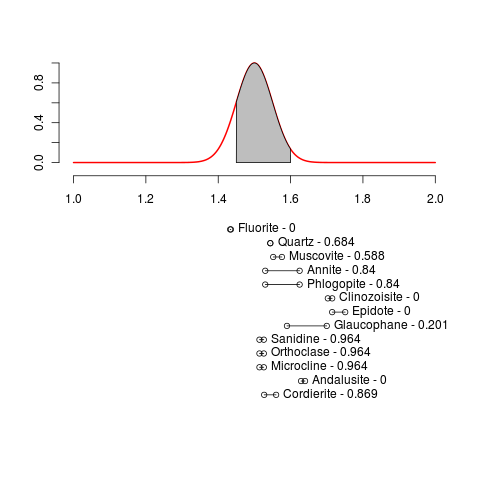
\includegraphics[width=100mm]{sample.png}
\end{center}
The Image above helps us represent a possible equation for scoring characteristics more specifically with respect to \ira. The user has provided us with:
\small
\begin{itemize}
\item[$\mu = $]$1.5$ denoting mean or best guess
\item[$\alpha =$]$1.45$ denoting lower bound on guess
\item[$\beta =$]$1.6$ denoting upper bound on guess
\end{itemize}
\normalsize

The distribution curve is representative of the normal distribution as expressed by:
\[f(x)=\frac{1}{\sqrt{2\pi\sigma^2}}\cdot e^{-\frac{(x-\mu)^2}{2\sigma^2}} \]
In this instance we choose (could easily be altered or made into piecewise)
\[\sigma=min(|\mu-\alpha|,|\mu-\beta|)\]
\begin{comment}
however
\[\sigma=max(|\mu-\alpha|,|\mu-\beta|)\]
or
\[\sigma=\frac{max(|\mu-\alpha|,|\mu-\beta|) + min(|\mu-\alpha|,|\mu-\beta|)}{2}\]

are also acceptable and could be argued to be preferable.
\end{comment}

The area defined by the shaded region is representative of the range addressed by the user, and the height is representative of how heavy the weighted score aught to be for a given mineral, whose \ira range is represented by unique lines below the graph.

Although it may be originally intuitive to use an integral equation to handle weighted scoring, there are several cases where one mineral's min and max of a specific attribute spans the entire domain. This can quickly throw off scores, so it is much more beneficial to just use the maximal value along the curve between the mineral's min and max.


\section*{\RangeA Scoring}
\begin{itemize}
\item Every attribute $a$ has what we have called it's characteristic number $\phi(a)$. This is a number that denotes how representative of minerals an attribute is. 
\item $M_i$ denotes the selected mineral.
\item Every mineral has $R(M_i,a)$  which is the min and max value tied to the specific \p{attribute}{mineral}. 
\item $S(M_i)$ denotes a specific mineral's accumulated score
\end{itemize}
The score awarded to minerals by \RangeA{}s is:

\[S(M_i) = \sum_{a\in Attributes} \left[ \phi(a) \cdot max \left(\frac{1}{f(\mu)}\cdot\frac{1}{\sqrt{2\pi{\sigma_a}^2}}\cdot e^{-\frac{(x-\mu_a)^2}{2{\sigma_a}^2}},\textrm{ $x\in$ range $(R(M_i,a) \cap \alpha(a)..\beta(a))$ }\right) \right] \]

Because there are at most {\bf 5} unique comparable values per \p{mineral}{attribute}, there exist trivial ways to cut time on this computation.

To facilitate an easier UI, it would be advantageous to allow the user to just place in their best guess, then use predetermined $\alpha(a)$ and  $\beta(a)$.
\pagebreak
\section*{Flow Chart}
The returned array has every relevent mineral, their total scores, and their catagorical scores.

\begin{itemize}
\item All Minerals start with a score of zero
\item {\bf \FP \& Marking} is done using the rules from the \EnumA{}s
\item {\bf \EnumA Scoring} is completed by adding the $\phi(a)$ of the \EnumA $a$ to the Mineral's Score
\item {\bf \RangeA Scoring} is done using values generated by the equation in the \RangeA Scoring Section
\end{itemize}
\begin{center}
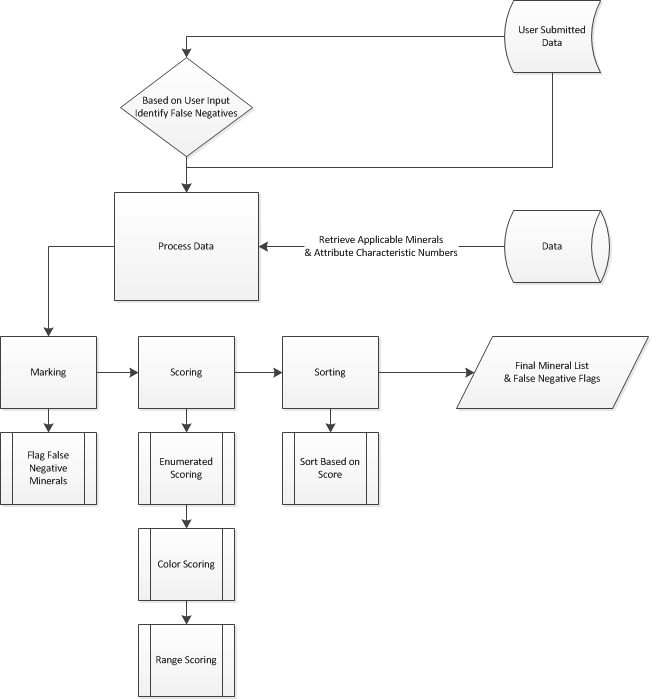
\includegraphics[width=80mm]{algFlowChart.png}
\end{center}
If the user requests $N$ minerals to be returned. Then the returned sorted array should contain $N$ elements that are specifically not \FP. In other words, assuming the lowest score of the $N$ requested minerals is 9:
\begin{itemize}
\item[{\bf if}] mineral R has score 20
\item[{\bf and}] mineral S has score 9
\item[{\bf and}] mineral R is marked \FP
\begin{itemize}
\item[{\bf then}] S counts towards the $N$ requested minerals
\item[{\bf and}] R does not count towards the requested $N$ minerals
\item[{\bf however}] R is returned in the final array, so users can dynamically switch between displaying \FP
\item[{\bf also}] any mineral Q with equivalent minimal scores $(score(Q)=score(S))$ should be returned as well, and displayed regardless of user specifications because they are computationally identical.
\end{itemize}
\end{itemize}
\end{document}
